% AER-Article.tex for AEA last revised 22 June 2011
\documentclass[AER]{AEA}

\usepackage{graphicx}

% The mathtime package uses a Times font instead of Computer Modern.
% Uncomment the line below if you wish to use the mathtime package:
%\usepackage[cmbold]{mathtime}
% Note that miktex, by default, configures the mathtime package to use commercial fonts
% which you may not have. If you would like to use mathtime but you are seeing error
% messages about missing fonts (mtex.pfb, mtsy.pfb, or rmtmi.pfb) then please see
% the technical support document at http://www.aeaweb.org/templates/technical_support.pdf
% for instructions on fixing this problem.

% Note: you may use either harvard or natbib (but not both) to provide a wider
% variety of citation commands than latex supports natively. See below.

% Uncomment the next line to use the natbib package with bibtex 
%\usepackage{natbib}

% Uncomment the next line to use the harvard package with bibtex
%\usepackage[abbr]{harvard}

% This command determines the leading (vertical space between lines) in draft mode
% with 1.5 corresponding to "double" spacing.
\draftSpacing{1.5}

\begin{document}

\title{Can We Ease the Reporting Decision? Investigating the Effects of Prominent Assault Cases on Sexual Assault Reporting}
\shortTitle{Sexual Assault Reporting}
\author{Harry Elworthy\thanks{Elworthy: Duke University, 837 Clarendon St Durham NC, harryelworthy@gmail.com.}}
\date{\today}
\pubMonth{}
\pubYear{}
\pubVolume{}
\pubIssue{}
\JEL{}
\Keywords{}

\begin{abstract}
Your abstract here.
\end{abstract}


\maketitle

American Economic Review Pointers:

\begin{itemize}
\item Do not use an "Introduction" heading. Begin your introductory material
before the first section heading.

\item Avoid style markup (except sparingly for emphasis).

\item Avoid using explicit vertical or horizontal space.

\item Captions are short and go below figures but above tables.

\item The tablenotes or figurenotes environments may be used below tables
or figures, respectively, as demonstrated below.

\item If you have difficulties with the mathtime package, adjust the package
options appropriately for your platform. If you can't get it to work, just
remove the package or see our technical support document online (please
refer to the author instructions).

\item If you are using an appendix, it goes last, after the bibliography.
Use regular section headings to make the appendix headings.

\item If you are not using an appendix, you may delete the appendix command
and sample appendix section heading.

\item Either the natbib package or the harvard package may be used with bibtex.
To include one of these packages, uncomment the appropriate usepackage command
above. Note: you can't use both packages at once or compile-time errors will result.

\end{itemize}

\clearpage

College sexual assault is an unavoidable topic on any campus. It is estimated that 20 - 25\% of women nationally report being sexually assaulted at some point during their college careers (Fisher, Cullen and Turner, 2000). At Duke, this figure is closer to 40\%, as well as 10\% of men (Fox, 2017). Despite this, very few assaults are reported to police or to universities, for a number of reasons. A number of different measures have been taken by many schools to address campus sexual assault, but there is little evidence on how effective these reforms have been at reducing assault or creating a better environment for victims. 

The 'Dear Colleague' letter of 2011 , released by the Office of Civil Rights (OCR), was a sizable shift in federal policy around campus sexual assault and the responsibility universities have to investigate allegations (Ali, 2011). It aimed to make reporting easier for an assault victim in a number of ways. For example, it reduced standards of evidence required in on-campus investigations, hopefully decreasing the chance of reporting an assault and having nothing happen. 

This paper finds a sizeable increase in report rates after 2011, across all post-secondary institutions. I summarize the data, looking at how report rates vary by tuition, racial makeup, and other variables.

I will then attempt to break down the increase, looking at different potential avenues through which the increase could be driven. These include the change in evidence standards referenced above, as well as changes in levels of national and local discourse on sexual assault, and changes in stringency in mandatory reporting standards.

In doing so, I will estimate a number of parameters that I hope will expand understanding on the effectiveness of various policies aimed at making reporting sexual assault an easier decision.


\section{Background}

The background section of Lindo et al. (2018b) provides a more complete background to the 'Dear Colleague' letter and its effects - here I will summarize their points. 

Title IX of the Education Amendments of 1972 was intended to 'assure equal access to education,' originally focused on female college sport. It has been reinterpreted in the form of 'Dear Colleague' letters, which are sent by the OCR, and allow slight changes in the law without congressional approval by framing the changes as 'clarifications'. The 2011 letter that this paper will focus on stated that Title IX required, among other things, that:

\begin{itemize}

\item If a school knew or "reasonably should know" of sexual harassment or assault, it was to conduct a "prompt, thorough, and impartial" investigation (Ali, 2011).

\item These investigations would use a "preponderance of evidence standard," which requires less proof than the standards of normal courts (Lindo et al., 2018b)

\item If the investigation found that sexual harassment or assault had occurred, the school was to "take immediate action to eliminate the hostile environment, prevent its reoccurrence, and address its effects" (Ali, 2011). 

\end{itemize}

Any victim that felt these steps had not been taken could file a complaint with the OCR which would trigger an investigation by the OCR into the way that school handled sexual harassment and assault. These cases are high profile, generating a large amount of press about the universities in question (Lindo et al., 2018b). 

In addition to these changes in 2011, the OCR made a number of further changes to policy in the following years, including putting more effort into getting mandatory reporters to report. Any employee of a university that receives federal funding is required to report to the school's Title IX coordinator any crime that is reported to them by a student, which will then be recorded in CSS statistics. In the years after 2011, the OCR increased efforts to enforce this rule . This enforcement could drive an increase in reports in the data without an actual increase in reports to staff.

These measures were taken in 2011 in response to a number of private documentaries and investigations that emphasized the nationwide injustices that victims face, the lack of repercussions for perpetrators and difficulty victims face while reporting. One key metric, then, to evaluate how well the policy has worked is report rates before and after the Letter was released. When reporting, a victim faces the choice of reporting to the police or to the university. A police report will usually lead to an investigation that is hugely costly to both the victim and the accused - something that most victims wish to avoid. Before 2011, a university report would lead to a number of different outcomes at different universities, but usually there would be an investigation that was still costly especially to the victim. The intention of the changes in 2011 were to make this university investigation less difficult for the victim. This paper will look at how this change in university investigation procedures has affected the reporting rates of victims both to universities and to the police.

The issue of non-reporting has been especially salient over the past weeks, as Supreme Court nominee Brett Kavanaugh has been accused of crimes that were not reported at the time. President Trump tweeted in response to the claims: "I have no doubt that, if the attack on Dr. Ford was as bad as she says, charges would have been immediately filed with local Law Enforcement Authorities by either her or her loving parents" (2018). While this tweet displays a woeful ignorance of the many reasons why an individual may not report, it illustrates a source of motivation for this paper: had Dr. Ford reported when the crime had been committed, her testimony now would be more impervious to detractors. There are many reasons that increased reporting would be a desirable outcome - this is just one of them. 

\section{Literature Review}

Since Becker outlined his economic model of crime, illicit activities have continued to have a place in the economic literature. Sexual assault has received a share of this attention, although perhaps less so than other crimes. One reason for this deficit is the difficulty of gathering accurate data on sexual assault. Crime is underreported in general, sexual assault especially (Kilpatrick et al, 2007) (Fisher et al, 2000). Recently, however, several economics papers have focused on sexual assault and harassment. 

Allen (2007) investigates the factors that influence an individual's decision to report a rape to law enforcement using survey data from The National Sample of Rape Victims, completed in 1985 and released in 2000, and finds that victims will be more likely to report sexual assault given more 'social support and ancillary evidence associated with the crime.' This paper is important to this investigation as it shows that the decision to report is influenced by factors that may be affected by policy, and thus supports the notion that policy to ease the reporting process could be beneficial. It is also some of the only research done on what affects the individual's decision to report. Given that I will be diving deeper into reasons this decision may have been made more often after 2011, this seems especially important to my investigation.

Yung (2015) investigates the idea that universities undercount reports in order to save face.  Comparing report numbers from years before and after an audit by the OCR, the paper estimates a consistent 40\% uptick in reports by universities in the year of an audit, followed by a return to preexisting trends the year directly after an audit. This is relevant for my paper, as this undercounting could affect the accuracy of the CSS data I am using, although the homogeneity found in undercounting indicates that it should not lead to bad estimates.

Lindo, Siminski, and Swensen, (2018a) looks at the effect of partying culture on reports of sexual assault. Specifically, using the plausible exogeneity of Division 1 football games, the paper estimates the effects of increased partying that comes with such events on reports of rape to law enforcement. The authors find a 28\% increase in rape reports associated with game days. Estimates are higher when the opponent is a rival, when the game is a Home rather than Away game, and when the game is televised. This paper is useful as it is a recent, high profile economics paper on the causes of sexual assault on college campuses, and for its use of NBIRS data, which will allow my paper to make use of this data much more easily.

Lindo, Marcotte, Palmer, and Swensen, (2018) considers the effects of a Title IX investigation on a universities outcomes such as enrolment, applications, degree completion and donations. Their estimates show significant upticks in both enrolment and applications following an investigation, with no evidence of effects on degree completion or donations. As part of their analysis, they use Google Trends data as a proxy for public awareness of investigations, concluding that the investigations are indeed in the public spotlight, even while federal policy on sexual assault may not be. The paper has an in-depth background of the 2011 Title IX changes that is very useful for my paper, as well as being closely related in subject. 

\section{Data Summary and Initial Regressions}

The most important data source that this paper will use is Campus Safety and Security (CSS) data collected and distributed by the Department of Education . Under the Clery act, any university that uses federal student financial aid - which is almost every university in the US - must disclose details about the reports of crime that it receives every year. This data catalogues these reports by school, year and type of crime from 2005 to 2016. There are 7,663 unique universities that span the entire time span, including 1,096 with more than 5000 students and 563 with more than 10,000. In 2016, 8,991 sexual crimes were reported in total. Figure 1 and Figure 2 show the general trend of reports by year.  

\section{Figures}

\begin{figure}

\includegraphics[width=4.9in]{figures/school_reports.eps}

\caption{Caption for figure below.}
\begin{figurenotes}
Figure notes without optional leadin.
\end{figurenotes}
\begin{figurenotes}[Source]
Figure notes with optional leadin (Source, in this case).
\end{figurenotes}
\end{figure}

\section{Tables}

\begin{table}
\caption{Caption for table above.}

{
\def\sym#1{\ifmmode^{#1}\else\(^{#1}\)\fi}
\begin{tabular}{l*{1}{c}}
\hline\hline
            &\multicolumn{1}{c}{(1)}\\
            &\multicolumn{1}{c}{police\_pc}\\
\hline
school\_pc   &      0.0379         \\
            &    (0.0722)         \\
[1em]
\_cons      &    0.000921\sym{***}\\
            & (0.0000333)         \\
\hline
\(N\)       &        1476         \\
adj. \(R^{2}\)&      -0.166         \\
\hline\hline
\multicolumn{2}{l}{\footnotesize Standard errors in parentheses}\\
\multicolumn{2}{l}{\footnotesize \sym{*} \(p<0.05\), \sym{**} \(p<0.01\), \sym{***} \(p<0.001\)}\\
\end{tabular}
}


\begin{tablenotes}
Table notes environment without optional leadin.
\end{tablenotes}
\begin{tablenotes}[Source]
Table notes environment with optional leadin (Source, in this case).
\end{tablenotes}
\end{table}

\begin{table}
\caption{Caption for table above.}

{
\def\sym#1{\ifmmode^{#1}\else\(^{#1}\)\fi}
\begin{tabular}{l*{3}{c}}
\hline\hline
            &\multicolumn{1}{c}{(1)}&\multicolumn{1}{c}{(2)}&\multicolumn{1}{c}{(3)}\\
            &\multicolumn{1}{c}{percap}&\multicolumn{1}{c}{percap}&\multicolumn{1}{c}{percap}\\
\hline
lead2       &   0.0000530\sym{*}  &                     &   0.0000530\sym{*}  \\
            & (0.0000207)         &                     & (0.0000207)         \\
[1em]
lead1       &    0.000137\sym{***}&                     &    0.000137\sym{***}\\
            & (0.0000210)         &                     & (0.0000210)         \\
[1em]
yof         &    0.000147\sym{***}&                     &    0.000147\sym{***}\\
            & (0.0000226)         &                     & (0.0000226)         \\
[1em]
lag1        &    0.000218\sym{***}&                     &    0.000218\sym{***}\\
            & (0.0000242)         &                     & (0.0000242)         \\
[1em]
lag2        &    0.000320\sym{***}&                     &    0.000320\sym{***}\\
            & (0.0000275)         &                     & (0.0000275)         \\
[1em]
after\_2011  &                     &    0.000259\sym{***}&    0.000234\sym{***}\\
            &                     & (0.0000115)         & (0.0000115)         \\
[1em]
\_cons      &    0.000123\sym{***}&    0.000123\sym{***}&    0.000123\sym{***}\\
            &(0.00000799)         &(0.00000808)         &(0.00000799)         \\
\hline
\(N\)       &       12887         &       12887         &       12887         \\
adj. \(R^{2}\)&      -0.134         &      -0.160         &      -0.134         \\
\hline\hline
\multicolumn{4}{l}{\footnotesize Standard errors in parentheses}\\
\multicolumn{4}{l}{\footnotesize \sym{*} \(p<0.05\), \sym{**} \(p<0.01\), \sym{***} \(p<0.001\)}\\
\end{tabular}
}


\begin{tablenotes}
Table notes environment without optional leadin.
\end{tablenotes}
\begin{tablenotes}[Source]
Table notes environment with optional leadin (Source, in this case).
\end{tablenotes}
\end{table}

\begin{table}
\caption{Caption for table above.}

{
\def\sym#1{\ifmmode^{#1}\else\(^{#1}\)\fi}
\begin{tabular}{l*{1}{c}}
\hline\hline
            &\multicolumn{1}{c}{(1)}\\
            &\multicolumn{1}{c}{school\_pc}\\
\hline
lead2       &  -0.0000329         \\
            & (0.0000234)         \\
[1em]
lead1       &  -0.0000432         \\
            & (0.0000234)         \\
[1em]
yof         &  -0.0000475         \\
            & (0.0000249)         \\
[1em]
lag1        &  -0.0000575\sym{*}  \\
            & (0.0000260)         \\
[1em]
lag2        &  -0.0000465         \\
            & (0.0000288)         \\
[1em]
\_cons      &    0.000106\sym{***}\\
            &(0.00000950)         \\
\hline
\(N\)       &        6309         \\
adj. \(R^{2}\)&       0.022         \\
\hline\hline
\multicolumn{2}{l}{\footnotesize Standard errors in parentheses}\\
\multicolumn{2}{l}{\footnotesize \sym{*} \(p<0.05\), \sym{**} \(p<0.01\), \sym{***} \(p<0.001\)}\\
\end{tabular}
}


\begin{tablenotes}
Table notes environment without optional leadin.
\end{tablenotes}
\begin{tablenotes}[Source]
Table notes environment with optional leadin (Source, in this case).
\end{tablenotes}
\end{table}

\begin{table}
\caption{Caption for table above.}

{
\def\sym#1{\ifmmode^{#1}\else\(^{#1}\)\fi}
\begin{tabular}{l*{1}{c}}
\hline\hline
            &\multicolumn{1}{c}{(1)}\\
            &\multicolumn{1}{c}{county\_pc}\\
\hline
lead2       &  -0.0000932         \\
            &  (0.000262)         \\
[1em]
lead1       &  -0.0000685         \\
            &  (0.000333)         \\
[1em]
yof         & 0.000000416         \\
            &  (0.000390)         \\
[1em]
lag1        &    0.000118         \\
            &  (0.000432)         \\
[1em]
lag2        &    0.000154         \\
            &  (0.000587)         \\
[1em]
\_cons      &    0.000664\sym{***}\\
            &  (0.000143)         \\
\hline
\(N\)       &       18094         \\
adj. \(R^{2}\)&      -0.078         \\
\hline\hline
\multicolumn{2}{l}{\footnotesize Standard errors in parentheses}\\
\multicolumn{2}{l}{\footnotesize \sym{*} \(p<0.05\), \sym{**} \(p<0.01\), \sym{***} \(p<0.001\)}\\
\end{tabular}
}


\begin{tablenotes}
Table notes environment without optional leadin.
\end{tablenotes}
\begin{tablenotes}[Source]
Table notes environment with optional leadin (Source, in this case).
\end{tablenotes}
\end{table}

\begin{table}
\caption{Caption for table above.}

{
\def\sym#1{\ifmmode^{#1}\else\(^{#1}\)\fi}
\begin{tabular}{l*{4}{c}}
\hline\hline
            &\multicolumn{1}{c}{(1)}&\multicolumn{1}{c}{(2)}&\multicolumn{1}{c}{(3)}&\multicolumn{1}{c}{(4)}\\
            &\multicolumn{1}{c}{reports}&\multicolumn{1}{c}{reports}&\multicolumn{1}{c}{reports}&\multicolumn{1}{c}{reports}\\
\hline
b\_norm      &      -0.995\sym{**} &      -0.628         &      -0.664         &     -0.0483         \\
            &     (0.352)         &     (0.338)         &     (0.387)         &     (1.558)         \\
[1em]
lag1        &                     &                     &     -0.0189         &                     \\
            &                     &                     &     (0.425)         &                     \\
[1em]
lag2        &                     &                     &       0.104         &                     \\
            &                     &                     &     (0.355)         &                     \\
[1em]
r\_norm      &                     &                     &                     &      -0.565         \\
            &                     &                     &                     &     (1.424)         \\
[1em]
SA\_norm     &                     &                     &                     &      0.0402         \\
            &                     &                     &                     &     (0.365)         \\
[1em]
\_cons      &       806.3\sym{***}&       654.6\sym{***}&       662.1\sym{***}&       651.5\sym{***}\\
            &     (23.51)         &     (33.35)         &     (39.90)         &     (35.01)         \\
\hline
\(N\)       &         626         &         626         &         624         &         626         \\
adj. \(R^{2}\)&       0.011         &       0.596         &       0.592         &       0.595         \\
\hline\hline
\multicolumn{5}{l}{\footnotesize Standard errors in parentheses}\\
\multicolumn{5}{l}{\footnotesize \sym{*} \(p<0.05\), \sym{**} \(p<0.01\), \sym{***} \(p<0.001\)}\\
\end{tabular}
}


\begin{tablenotes}
Table notes environment without optional leadin.
\end{tablenotes}
\begin{tablenotes}[Source]
Table notes environment with optional leadin (Source, in this case).
\end{tablenotes}
\end{table}

\begin{table}
\caption{Caption for table above.}

{
\def\sym#1{\ifmmode^{#1}\else\(^{#1}\)\fi}
\begin{tabular}{l*{3}{c}}
\hline\hline
            &\multicolumn{1}{c}{(1)}&\multicolumn{1}{c}{(2)}&\multicolumn{1}{c}{(3)}\\
            &\multicolumn{1}{c}{reports}&\multicolumn{1}{c}{reports}&\multicolumn{1}{c}{reports}\\
\hline
b\_norm      &      -0.119         &     0.00690         &       0.138         \\
            &    (0.0640)         &     (0.116)         &     (0.134)         \\
[1em]
bn\_norm     &                     &     -0.0230         &     -0.0444         \\
            &                     &    (0.0238)         &    (0.0270)         \\
[1em]
lag1        &                     &                     &     -0.0723         \\
            &                     &                     &     (0.142)         \\
[1em]
lag2        &                     &                     &      -0.194         \\
            &                     &                     &     (0.116)         \\
[1em]
n\_lag1      &                     &                     &      0.0139         \\
            &                     &                     &    (0.0291)         \\
[1em]
n\_lag2      &                     &                     &      0.0443         \\
            &                     &                     &    (0.0268)         \\
[1em]
\_cons      &       29.46\sym{***}&       24.87\sym{***}&       35.50\sym{***}\\
            &     (5.576)         &     (7.251)         &     (8.763)         \\
\hline
\(N\)       &         470         &         261         &         259         \\
adj. \(R^{2}\)&       0.404         &       0.303         &       0.274         \\
\hline\hline
\multicolumn{4}{l}{\footnotesize Standard errors in parentheses}\\
\multicolumn{4}{l}{\footnotesize \sym{*} \(p<0.05\), \sym{**} \(p<0.01\), \sym{***} \(p<0.001\)}\\
\end{tabular}
}


\begin{tablenotes}
Table notes environment without optional leadin.
\end{tablenotes}
\begin{tablenotes}[Source]
Table notes environment with optional leadin (Source, in this case).
\end{tablenotes}
\end{table}


References here (manual or bibTeX). If you are using bibTeX, add your bib file 
name in place of BibFile in the bibliography command.
% Remove or comment out the next two lines if you are not using bibtex.
\bibliographystyle{aea}
\bibliography{BibFile}

% The appendix command is issued once, prior to all appendices, if any.
\appendix

\section{Mathematical Appendix}

\end{document}

